\chapter{Grundlagen} \label{sm-ansaetze}
% TODO Aufbau überarbeiten, weniger Subsections

Bei den populären \acrshort{ac:sm} Lösungen folgen Redux und NgRx dem Flux-Pattern\cite{historyOfRedux}\cite{ngrxGettingStarted}, wobei Zustand und Pinia einen anderen, Framework-nahen Ansatz verfolgen. Im Folgenden wird die Funktionsweise und die Eigenschaften von Redux und Pinia näher beschrieben, da diese grundlegend unterschiedliche Ansätze verfolgen und andere \acrshort{ac:sm} Lösungen sich einem der beiden ähneln.

\section{Redux}

Redux definiert sich durch folgende vier Eigenschaften:
\begin{enumerate}
  \item Unveränderlichkeit (Immutability): Änderungen am State sind ausschließlich über die APIs von Redux unter Beachtung der Unveränderlichkeit möglich.
  \item Zentralisierung des Zustandes: Der gesamte Applikationszustand lebt in einem zentralen JavaScript Objekt.
  \item Nachvollziehbarkeit (Traceability): Während der gesamten Lebensdauer der Applikation sind Änderungen am Zustand auf deren Ursprung verfolgbar.
  \item Event-basiert: Es wird das Beobachter-Muster (Observer Pattern) verwendet.
\end{enumerate}

Das Verhalten des Stores wird durch \textit{actions} und \textit{reducer} definiert.
% Außerdem können optionale \textit{selectors} benutzt werden, um aus bestimmten Teilen des Zustandes zu lesen.

\subsection{Actions}

Eine Aktion (Action) beschreibt eine Änderung oder Interaktion in und mit der Applikation. Beispielsweise könnte eine \textit{counter-clicked} Action versendet (dispatch) werden, wenn der Nutzer auf den \textit{Zähler erhöhen}-Button drückt. Oder, wenn der Nutzer sich erfolgreich angemeldet hat, kann eine entsprechende Action versendet werden. Intern ist eine Action ein \acrshort{ac:pojo}.\cite{reduxStateActionReducers}

Es wird folgende Struktur für Actions empfohlen:
\begin{lstlisting}
type Action<T> = {
  type: string,
  payload?: T
}
\end{lstlisting}

Das Feld \textit{type} beschreibt die Action, und das optionale Feld \textit{payload} enthält weiterführende Daten.

\subsection{Reducer}

Der Reducer ist für die Initialisierung und Aktualisierung des Zustandes zuständig. Er wird als eine Pure-Function mit zwei Parametern definiert.
Der erste Parameter ist das Zustandsobjekt und der zweite die versendete Action. Der Rückgabewert dieser Funktion ist das neue Zustandsobjekt. Da es sich hier um eine Pure-Function handelt, dürfen keine Seiteneffekte stattfinden. Wie eingangs erwähnt, ist der Zustand unveränderlich, daher dürfen hier keine direkten Veränderungen des Zustandes stattfinden. Es wird lediglich ein neues Objekt zurückgegeben. Falls keine Veränderungen stattfinden sollen, kann das ursprüngliche Objekt aus dem ersten Parameter unverändert zurückgegeben werden.\cite{reduxStateActionReducers}

Es wird folgende Struktur für Reducer empfohlen:
\begin{lstlisting}
type Reducer<S, A> = (state: S, action: A) => S
\end{lstlisting}

Beispiel-Reducer:

\begin{lstlisting}
function reducer(state = { user: null }, action) {
  switch (action.type) {
    case 'user-logged-in':
      return {
        ...state,
        user: {
          userId: action.payload.userId
        },
      }
    case 'user-logged-out':
      return {
        ...state,
        user: null,
      }
    default:
      return state
  }
}
\end{lstlisting}

Es wird die \textit{Spread-Syntax: ...} aus ECMAScript 6 genutzt, um das ursprüngliche Zustandsobjekt zu kopieren (shallow copy).\cite{mdnSpreadSyntax}

\subsection{Definition und Interaktion mit dem Store}

Der Store wird mit Hilfe der \textit{createStore}-API erstellt. Als Parameter wird die Reducer-Function übergeben. Der Rückgabewert ist das Store-Objekt. Dieses bietet Zugang zu unter anderem \textit{dispatch} und \textit{getState}-Methoden. Mit diesen kann jeweils eine Action versendet und aus dem Store gelesen werden.

\begin{lstlisting}
const store = createStore(reducer)
store.dispatch(action)
const user = store.getState().user
\end{lstlisting}

Die erwähnten Redux-APIs sind die Grundlage für den unidirektionalen Datenfluss in Redux, wie in Abb. \ref{fig:redux-dataflow} dargestellt.

\begin{figure}[H]
  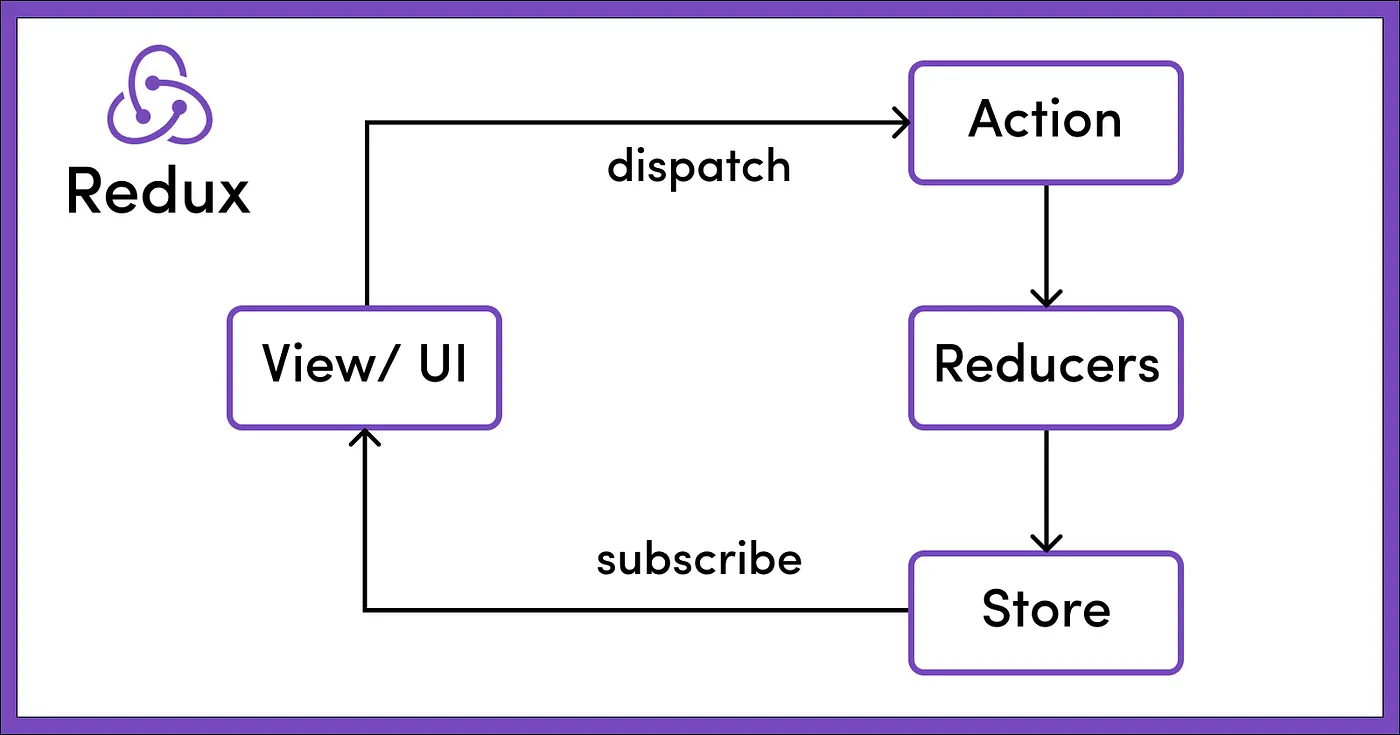
\includegraphics[width=1\textwidth]{redux-dataflow.png}
  \caption{How to use Redux architecture — Part 1 [\citeyear{reduxDataFlow}]}
  \label{fig:redux-dataflow}
\end{figure}

\section{Pinia}

Pinia ist sehr eng gekoppelt mit dem Vue-Framework und nutzt dessen Mechanismen der Reaktivität zur Datenhaltung. Das führt dazu, dass Pinia selbst minimal bleibt und die Daten ohne Weiteres reaktiv sind. Im Gegensatz zu Redux und NgRx setzt diese Store-Lösung nicht das Flux-Pattern um. Dank dieser Praxis ist weniger Code nötig, um einen Store zu definieren. Außerdem folgt Pinia nicht dem Single-Store-Ansatz, bei dem alle Daten in einem zentralen Objekt leben, sondern es sind für Teile der Daten eigenständige Store-Instanzen zuständig. Pinia bietet zwei verschiedene APIs zur Definition von Stores an. In dieser Arbeit wird die \textit{Options API} verwendet. Die Konzepte lassen sich auch auf die \textit{Composition API} übertragen.\cite{piniaDefiningAStore} Die zwei essentiellen Konzepte sind \textit{State} und \textit{Action}.

\subsection{State}

State ist eine Funktion, die ein Objekt zurückgibt, das den Zustand enthält.

\subsection{Action}

Eine Action ist eine Methode, die den State verändert und in einem \textit{actions}-Objekt definiert wird.

\subsection{Definition eines Stores}

Zur Definition eines Stores wird die \textit{defineStore}-API genutzt. Als Parameter wird ein eindeutiger Name und eine Beschreibung des Stores in Form eines Objekts übergeben. Im zweiten Parameter werden die Felder \textit{state} und \textit{actions} definiert.

\begin{lstlisting}
const useUserStore = defineStore('user-store', {
  state: () => {
    user: null
  },
  actions: {
    updateUser(newUser) {
      this.user = newUser
    }
  }
})
\end{lstlisting}

Auf die Felder im State-Objekt wird in einer Action mit \textit{this} zugegriffen. Das State-Objekt wird seitens Pinia intern jeder Action gebunden.

\subsection{Interaktion mit dem Store}

Der Store kann in einer beliebigen Vue-Komponente importiert werden. Die Felder des Objekts, das von der \textit{state}-Funktion zurückgegeben wird, werden automatisch zu Feldern des Store-Objekts. Genauso werden auch die Methoden des \textit{actions}-Objekts zu Membern des Store-Objekts.

\begin{lstlisting}
  const userStore = useUserStore()
  
  // userStore.user
  // userStore.updateUser
\end{lstlisting}

Der State im oberen Beispiel ist reaktiv und kann als \textit{userStore.user} im Template der Komponente referenziert werden. Die Destrukturierung (destructuring) des Store-Objekts, im oberen Beispiel \textit{userStore}, führt zum Verlust der Reaktivität. Aus diesem Grund wird die Punktnotation empfohlen.\cite{piniaDefiningAStore}
